\begin{table*}[t]
\centering\small
\setlength{\tabcolsep}{5pt}
\caption{First release: 2,000 tasks per method, ten models, 906 target references and 1,034 Spider items. Lower is better. Direct TEF differences share source unknowns; negative favors S2B. Unknowns count scores out of 20,000. Bold marks established improvements, comparing S2B with Template for absolute scores and with each stated comparator for differences.}
\label{tab:main}
\begin{tabular}{lrrrr}\toprule
Method & Target gap $G\downarrow$ & Spider--BIRD TEF $\downarrow$ & Direct $\Delta\mathrm{TEF}$ & Unknown\\\midrule
\multicolumn{5}{l}{\textit{Verified execution scoring}}\\
Template & $[0.224967, 0.224967]$ & $[0.243915, 0.390986]$ & $\boldsymbol{[-0.131730, -0.079099]}$ & 0\\
S2B & $\boldsymbol{[0.169275, 0.169275]}$ & $\boldsymbol{[0.138501, 0.283651]}$ & $0$ & 0\\
RingSQL-style adaptation & $[0.096309, 0.100791]$ & $[0.283403, 0.435663]$ & $\boldsymbol{[-0.233594, -0.061506]}$ & 46\\
OmniSQL component adaptation & $[0.029731, 0.134760]$ & $[0.564696, 0.862439]$ & $\boldsymbol{[-0.665769, -0.324655]}$ & 1,290\\
SynthSQL-style local adaptation & $[0.013004, 0.166928]$ & $[0.268596, 0.642072]$ & $\boldsymbol{[-0.453605, -0.021084]}$ & 2,040\\
\midrule
\multicolumn{5}{l}{\textit{Base layer: strict execution and output-shape checks}}\\
Template & $[0.178882, 0.262025]$ & $[0.205735, 0.426469]$ & $[-0.193294, +0.005344]$ & 430\\
S2B & $[0.117662, 0.208049]$ & $[0.111299, 0.334757]$ & $0$ & 537\\
RingSQL-style adaptation & $[0.059199, 0.138379]$ & $[0.241426, 0.462380]$ & $[-0.293401, +0.034557]$ & 445\\
OmniSQL component adaptation & $[0.010465, 0.190895]$ & $[0.488896, 0.898945]$ & $\boldsymbol{[-0.734008, -0.195186]}$ & 2,066\\
SynthSQL-style local adaptation & $[0.000000, 0.345368]$ & $[0.103282, 0.861883]$ & $[-0.686921, +0.198272]$ & 5,149\\
\bottomrule
\end{tabular}
\end{table*}
\begin{figure*}[t]
\centering
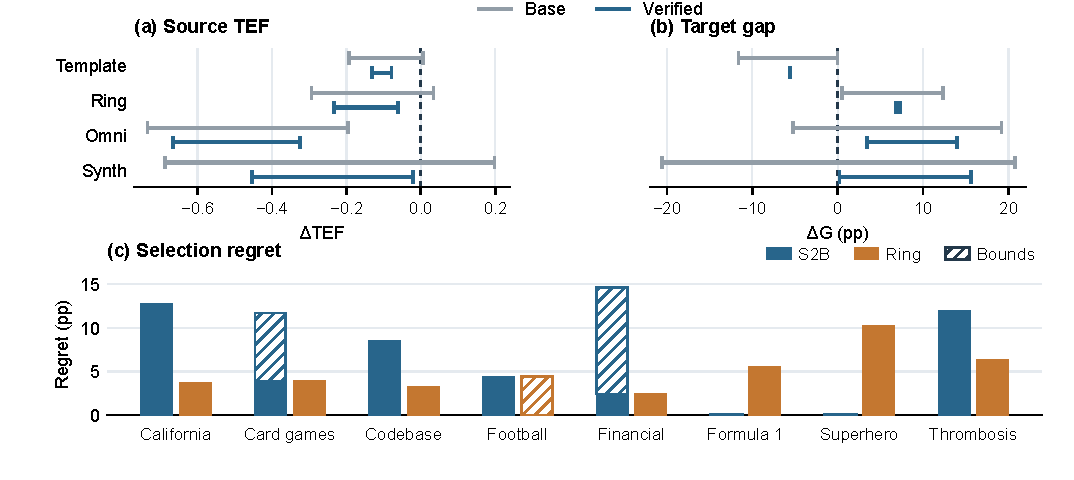
\includegraphics[width=\textwidth]{figures/current/Fig3.pdf}
\caption{First-release source TEF, target gap and model-selection regret. Panels (a--b) compare S2B with each method; panel (c) compares S2B and Ring by domain. Caps indicate bounds; ticks indicate coincident endpoints.}
\label{fig:main-contrasts}
\end{figure*}
